For the purpose of showing some functionality to potential customers of the solution, it was chosen to construct a vertical prototype of the smartphone application.

The prototype implemented some of the key functionality, still leaving some functionality. The purpose of this is to show a small set of complete functionality. The application was supposed to look like the paper prototype described in \cref{paper_prototype}. Some of the design functionality were not implemented or replaced with a dummy button just to show the potential design.

\begin{figure}[hbtp]
  \centering
  \subfloat[An example search in the prototype.]{
    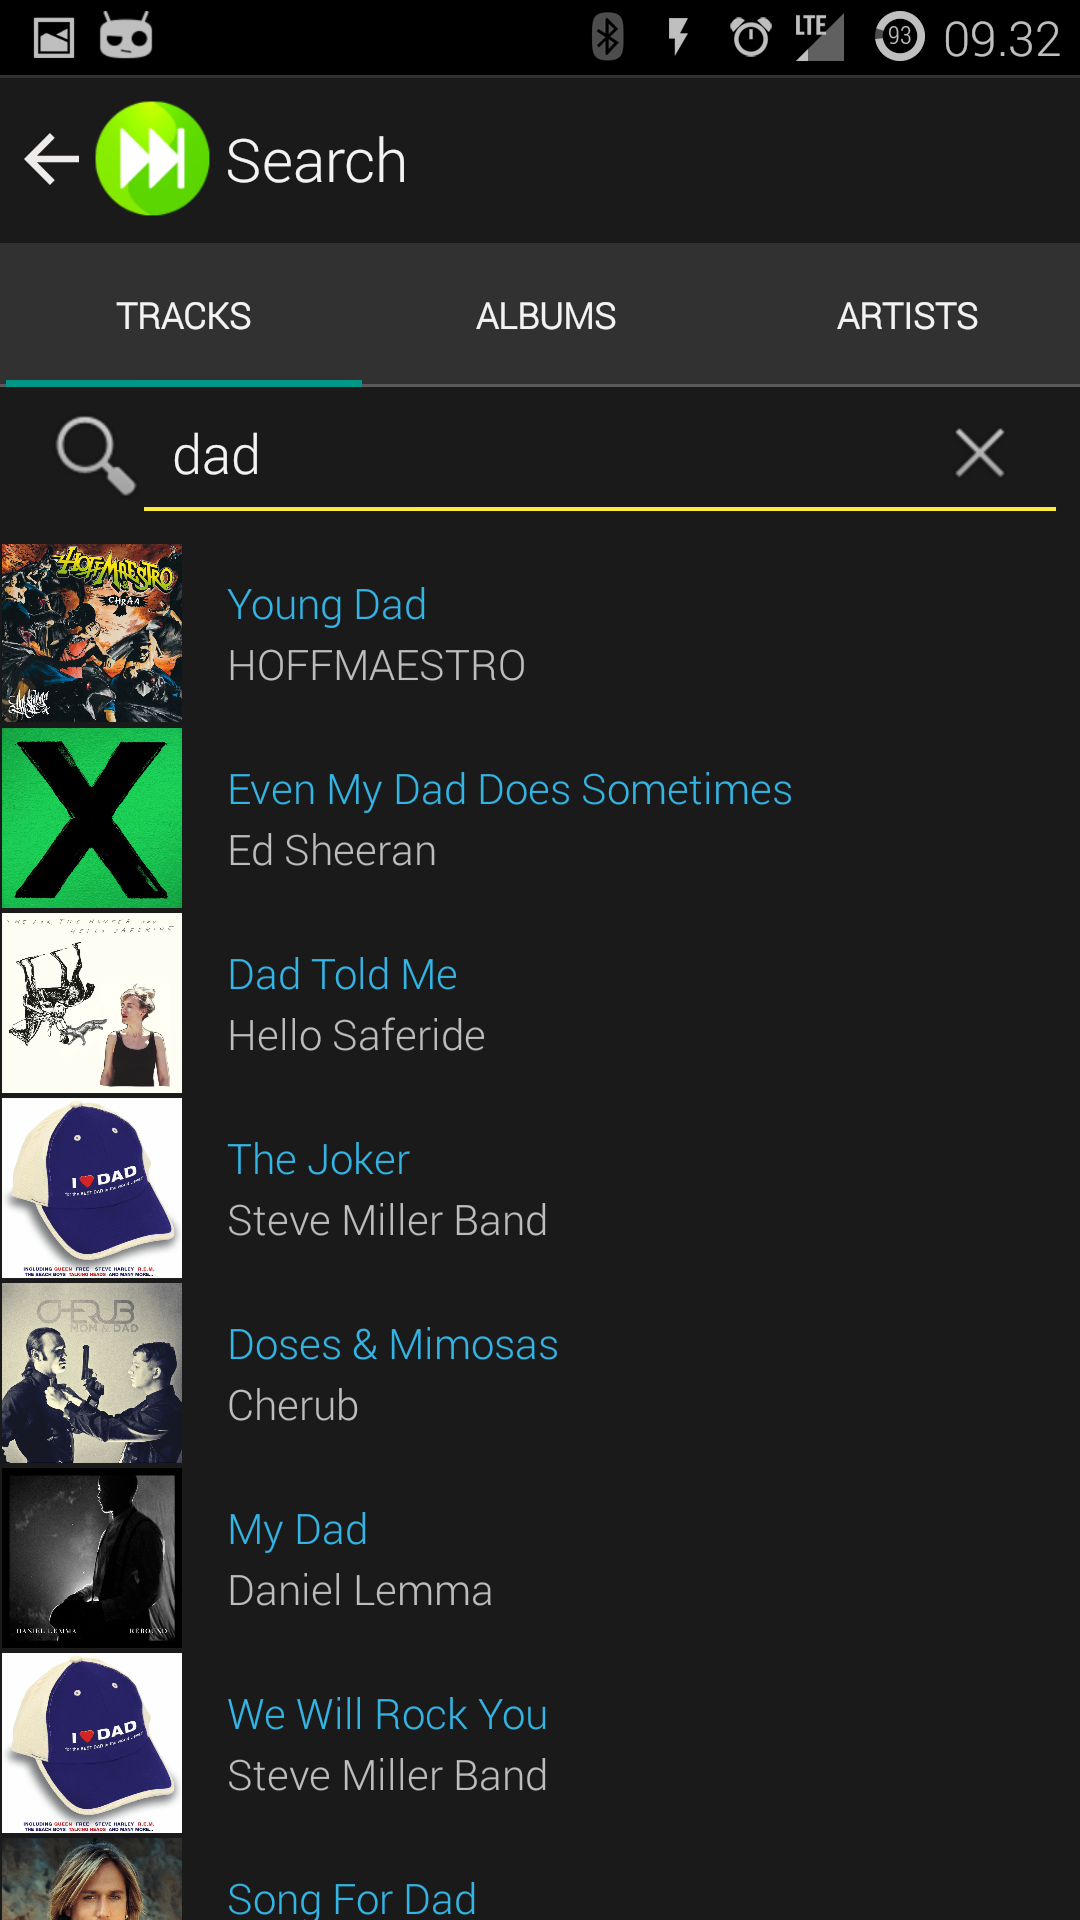
\includegraphics[width=0.5\textwidth]{searchResult}
    \label{fig:searchResult}
  }
  \subfloat[In this early prototype the user still needed to enter the IP manually.]{
    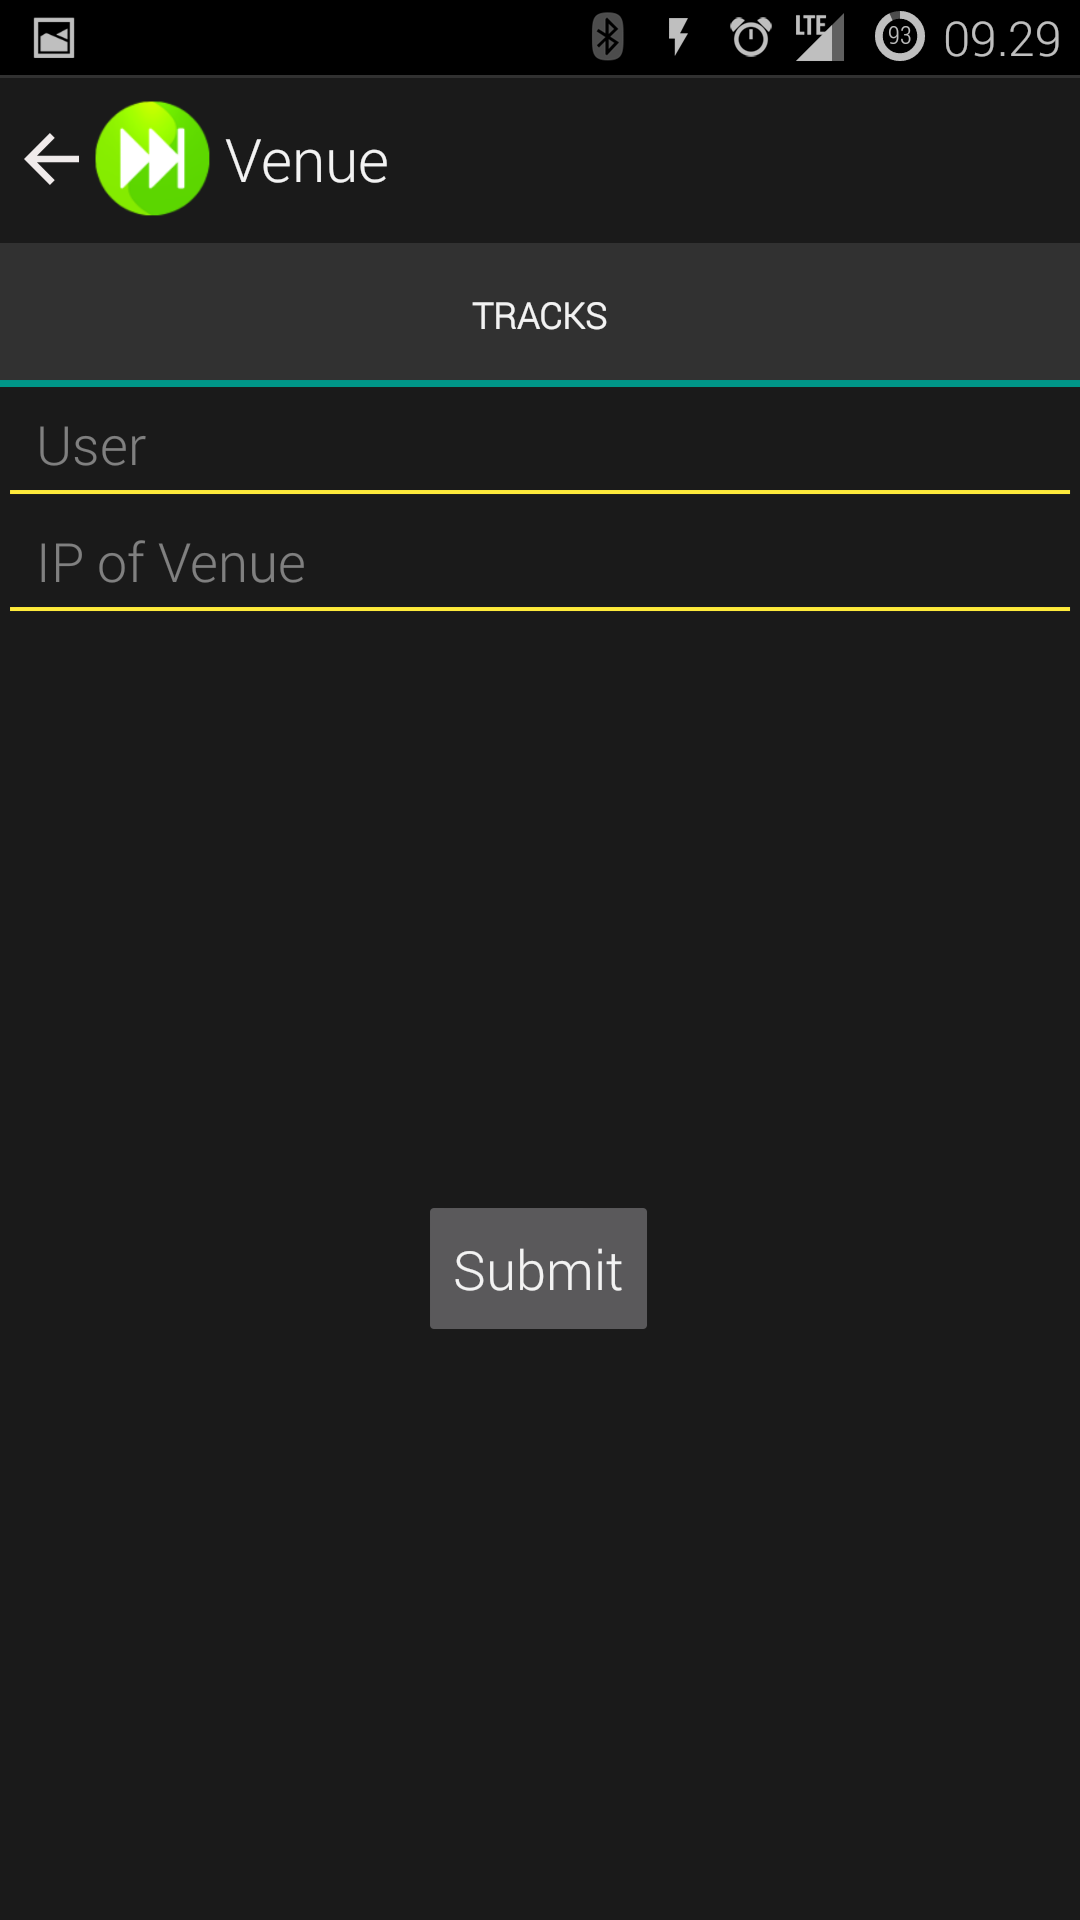
\includegraphics[width=0.5\textwidth]{ipScreen}
    \label{fig:ipScreen}
  }
  \caption{Screenshots from the prototype shown to \enquote{Fabrikken}.}
\end{figure}

\subsection{Vertical Prototype}
\label{sub:vertical_prototype}

The prototype was designed for android phones, which is one of the mobile platforms that the application is supposed to support. The prototype was suppose to show some of the key functionalities like, the search functionality shown at \cref{fig:searchResult}. The prototype implemented simple functionality that enabled users to vote on a track and send the request to the server. In this prototype the way users check's in at a bar was to type in the ip of the bar's server and a username, as shown at \cref{fig:ipScreen}. This was an acceptable prototype because the focus was on the playback and search functionality.